\documentclass[11pt]{article}
\usepackage{geometry}
\geometry{
  a4paper,
  left=30mm,
  right=30mm,
  top=30mm,
  bottom=30mm
  }
\usepackage{amsmath, amssymb, amsthm}
\usepackage{bm, graphicx}
\usepackage[colorlinks=true]{hyperref}
\usepackage[backend=biber]{biblatex}
\addbibresource{ref.bib}
\usepackage{algorithm}
\usepackage{algpseudocode}
\usepackage{booktabs}
\usepackage{pifont}
\usepackage{multirow}
\usepackage{tikz}
\usetikzlibrary{arrows.meta, positioning, decorations.pathreplacing}

\newcommand{\cmark}{\ding{51}}
\newcommand{\xmark}{\ding{55}}

\newtheorem{theorem}{Theorem}
\newtheorem{definition}{Definition}
\newtheorem{proposition}{Proposition}
\newtheorem{remark}{Remark}
\newtheorem{corollary}{Corollary}
\newtheorem{requirement}{Requirement}
\newtheorem{assumption}{Assumption}

\newcommand{\R}{\mathbb{R}}
\newcommand{\Q}{\mathcal{Q}}
\newcommand{\Hilb}{\mathcal{H}}
\newcommand{\Tr}{\operatorname{Tr}}
\newcommand{\D}{\mathcal{D}}

\begin{document}

\title{Dynamics-Level Watermarking of Flow Matching Models with Random Codes}
\author{Shuchan Wang}
\date{\today}
\maketitle

\begin{abstract}
We introduce a dynamics-level approach to watermarking generative models.
Rather than embedding signals into model weights or outputs, we embed the
watermark directly into the learned continuous dynamics---the velocity
field of a flow matching model. We formulate this as random coding over a
continuous channel: a key-dependent perturbation is added during training,
and the message is recovered at detection time from black-box queries. The
perturbation is designed to leave the generated distribution unchanged.
Experiments on MNIST and CIFAR-10 across different architectures confirm
reliable message recovery, preserved generation quality, and chance-level
decoding accuracy without the secret key.
\end{abstract}

\section{Introduction}

\subsection{Background: Flow Matching Generative Models}

Flow matching~\cite{lipmanflow,liuflow} has emerged as a powerful framework
for training continuous normalizing flows. Given samples $x_1 \sim
q_{\text{data}}$ from a data distribution and $x_0 \sim p_{\text{noise}}$
from a simple base distribution, flow matching learns a time-dependent
velocity field $v_\theta(x,t)$ that transports $p_{\text{noise}}$ to
$q_{\text{data}}$ along the trajectory
\begin{equation}
\frac{dx_t}{dt} = v_\theta(x_t, t), \quad t \in [0,1].
\end{equation}
The model is trained by regressing $v_\theta$ against a conditional
velocity field $u(x_t|x_0,x_1)$ defined along interpolating paths
$x_t = (1-t)x_0 + t x_1$. At convergence, integrating the ODE from
$x_0 \sim p_{\text{noise}}$ produces samples $x_1 \sim q_{\text{data}}$.

The key object learned by flow matching is the velocity field
$v_\theta: \mathbb{R}^d \times [0,1] \to \mathbb{R}^d$, a continuous
function that completely characterizes the generative process. Training
such a model requires substantial computational resources, making the
resulting velocity field valuable intellectual property in need of
protection against unauthorized use.

\subsection{Requirements for Generative Model Watermarking}

A watermarking scheme for a generative model should satisfy the following
properties. The watermark should be embedded in the model itself, so that
it persists across different generated outputs and cannot be circumvented
simply by bypassing a post-processing step (model-level embedding).
Detection should require only query access to the model, without access to
weights, training data, or the generation pipeline, enabling verification
of deployed models accessible only through APIs (black-box
verifiability). Watermarked models should generate samples that are
statistically indistinguishable from those of unwatermarked models, with
no visible artifacts or degradation in fidelity (quality preservation).
Detection and message recovery should require knowledge of a secret key;
without the key, an attacker should be unable to recover the embedded
message beyond chance level (keyed security). Finally, the scheme
should support encoding a multi-bit message, enabling applications beyond
binary ownership verification, including owner identification, model
versioning, customer-specific serialization, and traitor tracing across
distributed copies (multi-bit capacity).

\subsection{Limitations of Existing Approaches}

We categorize existing watermarking methods by what they watermark.
Output-level methods embed signals into generated
samples~\cite{wen2023tree,fernandez2023stable}. These are not model-level:
removing the post-processing step eliminates the watermark, and they
provide no evidence of model ownership if the model itself is copied.
Weight-level methods embed bits into model
parameters~\cite{uchida2017embedding}. While model-level, they require
white-box access and are fragile to fine-tuning, pruning, or
quantization. Behavior-level methods use backdoor triggers---specific inputs that
produce predetermined outputs~\cite{adi2018turning,chen2019blackmarks,fei2025high}.
These methods operate at the model level and support black-box
verification. However, trigger-based approaches can introduce visible
artifacts or statistical irregularities, and often lack strong
cryptographic keying: once a trigger is discovered, any party can verify
the watermark. Recent work extends this to multi-bit payloads via channel
coding~\cite{fei2025high}.

Table~\ref{tab:comparison} in Appendix~\ref{app:comparison} summarizes how
existing paradigms compare against the five desiderata. To our knowledge,
no prior work embeds the watermark directly into the learned continuous
dynamics of the generative process itself. Existing black-box multi-bit
methods instead rely on trigger behaviors, output statistics, or
parameter-space embeddings, rather than perturbations of the transport
dynamics.

\subsection{The Gap: Dynamics-Level Watermarking}

In flow matching, the velocity field $v_\theta(x,t)$ is a continuous
function that defines the generative dynamics. This perspective reveals an underexplored opportunity: the velocity field can be viewed as a high-dimensional continuous channel into which information may be
embedded through structured perturbations, while preserving the overall
behavior of the model.

This gap motivates our core question:
\begin{quote}
\emph{Can we embed a verifiable, keyed, multi-bit message directly into
the learned velocity field of a flow matching model, such that (1) the
watermark is detectable with only black-box access, (2) generation
quality is preserved, and (3) reliable detection requires access to a
secret key?}
\end{quote}

\subsection{Our Approach and Contributions}

Our specific contributions are as follows. First, we formulate
watermarking directly at the level of the learned dynamics, embedding the
message as a key-dependent perturbation of the continuous velocity field
rather than into weights or outputs (model-level embedding). Second, we
design the perturbation to integrate to zero over each generative
trajectory, so that the terminal distribution of generated samples is
preserved in practice (quality preservation). Third, the watermark is keyed by a secret projection matrix and an orthogonal
codebook; without this key, empirical detection accuracy matches the random
guess rate (keyed security). Fourth, the scheme supports multi-bit messages via the codebook construction, enabling identification beyond binary verification (multi-bit capacity).
Fifth, we validate the method on MNIST and CIFAR-10 across MLP and UNet
architectures, achieving $100\%$ message recovery with chance-level
false positive rate, FID ratios $0.95\times$--$1.1\times$, and
statistical separation exceeding $8.4\sigma$ across all settings
(empirical validation). These properties make dynamics-level watermarking
a potential foundation for applications such as model ownership
verification, traitor tracing, and regulatory compliance, though we leave
their deployment-scale evaluation to future work.

\begin{figure}[t]
\centering
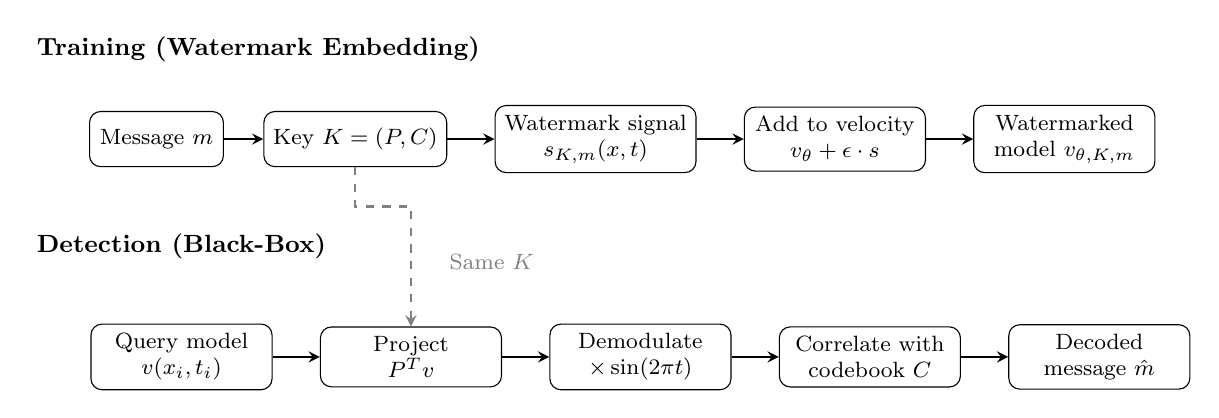
\begin{tikzpicture}[
    node distance=0.6cm,
    box/.style={rectangle, draw, rounded corners, minimum width=2.3cm, minimum height=0.7cm, align=center, font=\footnotesize},
    smallbox/.style={rectangle, draw, rounded corners, minimum width=1.7cm, minimum height=0.7cm, align=center, font=\footnotesize},
    arrow/.style={->, >=stealth, thick},
]

% ===== TRAINING PHASE =====
\node[font=\small\bfseries, anchor=west] (trainlabel) at (-5.5, 0) {Training (Watermark Embedding)};

\node[smallbox, below left=0.5cm and -2.5cm of trainlabel] (msg) {Message $m$};
\node[smallbox, right=0.5cm of msg] (key) {Key $K = (P, C)$};
\node[box, right=0.6cm of key] (signal) {Watermark signal\\$s_{K,m}(x,t)$};
\node[box, right=0.6cm of signal] (add) {Add to velocity\\$v_\theta + \epsilon \cdot s$};
\node[box, right=0.6cm of add] (model) {Watermarked\\model $v_{\theta,K,m}$};

\draw[arrow] (msg) -- (key);
\draw[arrow] (key) -- (signal);
\draw[arrow] (signal) -- (add);
\draw[arrow] (add) -- (model);

% ===== DETECTION PHASE =====
\node[font=\small\bfseries, anchor=west] (detlabel) at (-5.5, -2.5) {Detection (Black-Box)};

\node[box, below=0.7cm of detlabel] (query) {Query model\\$v(x_i, t_i)$};
\node[box, right=0.6cm of query] (proj) {Project\\$P^T v$};
\node[box, right=0.6cm of proj] (demod) {Demodulate\\$\times \sin(2\pi t)$};
\node[box, right=0.6cm of demod] (corr) {Correlate with\\codebook $C$};
\node[box, right=0.6cm of corr] (out) {Decoded\\message $\hat{m}$};

\draw[arrow] (query) -- (proj);
\draw[arrow] (proj) -- (demod);
\draw[arrow] (demod) -- (corr);
\draw[arrow] (corr) -- (out);

% ===== KEY REUSE ARROW =====
\draw[arrow, dashed, gray] (key.south) -- ++(0, -0.5) -| (proj.north);
\node[font=\footnotesize\color{gray}] at (0.4, -2.7) {Same $K$};

\end{tikzpicture}
\caption{Overview of the proposed dynamics-level watermarking framework.
\textbf{Top (Training):} A message $m$ and secret key $K$ define a
time-modulated watermark signal $s_{K,m}$, which is added to the velocity
field during flow matching. \textbf{Bottom (Detection):} Given black-box
access to a model, the detector projects velocity queries into the code
space, demodulates with the temporal carrier, and correlates against the
codebook to recover the embedded message. The same key $K$ is used for
embedding and detection.}
\label{fig:overview}
\end{figure}

%========================================================================
\section{Watermarking as Random Coding over Transport Dynamics}

In this section, we formalize our approach. We first describe the
information-theoretic motivation, then detail the construction of keys,
codes, and the time-modulated watermark, followed by the training and
detection procedures.

\subsection{Information-Theoretic Motivation}

From an information-theoretic perspective, our approach views the velocity
field as a continuous additive channel. Let $v_\theta(x,t)$ be the clean
velocity field and consider a watermarked version:
\begin{equation}\label{eq:vwm}
v_{\theta,K,m}(x,t) = v_\theta(x,t) + \eta(x,t) + \epsilon \cdot s_{K,m}(x,t),
\end{equation}
where $\eta(x,t)$ represents background variation from training
stochasticity and $s_{K,m}(x,t)$ is a key-dependent signal encoding
message $m$.

The detection problem becomes: given $N$ noisy observations of
$v_{\theta,K,m}(x_i,t_i)$, estimate $\hat{m}$ with high confidence.
This is a random coding problem over a continuous channel---a classical
setup in information theory \cite{cover1999elements} that guarantees
reliable decoding when the codebook is appropriately constructed and the
number of observations is sufficient.

\subsection{Message and Key: Framework}

Equation~\eqref{eq:vwm} reduces the watermarking problem to the
construction of the signal $s_{K,m}(x,t)$. We first give a general
formulation.

Let $m \in \mathcal{M}$ be a message from a set of
$|\mathcal{M}| := 2^L$ possible messages, and let $K$ be a secret key.
The key defines a codebook through a mapping
\begin{equation}
\phi_K : \mathcal{M} \to \mathcal{H},
\end{equation}
where $\mathcal{H}$ is a function space over $(x,t)$. The codeword for
message $m$ is $s_{K,m}(x,t) := \phi_K(m)$.

The design of $s_{K,m}$ must balance three considerations: (i) detectability---the signal must be recoverable from noisy observations
through a known detection procedure; (ii) quality preservation---the
signal must not alter the generated sample distribution, meaning it should
integrate to zero along trajectories; and (iii) security---without
knowledge of the key $K$, the watermark must be unrecoverable beyond chance level.

These considerations are formalized as the following three requirements
on the codebook.

\begin{definition}[Admissible codebook]\label{def:admissible}
A codebook $\{s_{K,m}\}_{m\in\mathcal{M}}$ is called \textbf{admissible}
if it satisfies the following conditions.
\begin{enumerate}
\item \textbf{Zero-mean over time.} For all $m \in \mathcal{M}$ and
all $x$,
\begin{equation}
\int_0^1 s_{K,m}(x,t) \, dt = 0.
\end{equation}
\item \textbf{Approximate orthogonality.} For any distinct
$m, m' \in \mathcal{M}$,
\begin{equation}
\langle s_{K,m}, s_{K,m'} \rangle \approx 0.
\end{equation}
\item \textbf{Energy normalization.} There exists a constant $C > 0$
such that for all $m \in \mathcal{M}$,
\begin{equation}
\|s_{K,m}\|^2 \approx C.
\end{equation}
\end{enumerate}
\end{definition}

Condition~1 ensures the watermark integrates to zero along trajectories,
preserving sample quality. Condition~2 ensures that different messages
are maximally separable at detection time. Condition~3 ensures that
all messages are equally detectable. These conditions are design
principles that guide our construction; they are neither necessary for
watermarking in general nor sufficient to guarantee empirical success.
We validate the practical performance of our construction in
Section~\ref{sec:experiments}.

\subsection{Concrete Construction}\label{sec:concrete}

We now present one construction satisfying
Definition~\ref{def:admissible}, chosen for its simplicity and exact
satisfaction of the orthogonality condition. Other choices are possible,
as discussed in Remark~\ref{rem:alternatives} below.

The secret key consists of two components, $K = (P, C)$. Here
$P \in \mathbb{R}^{D \times k}$ is a semi-orthogonal projection matrix
satisfying $P^T P = I_k$, generated by QR decomposition of a random matrix
seeded by $K$. This maps from the $D$-dimensional velocity space to a
$k$-dimensional latent code space. The component
$C = \{c_m\}_{m \in \mathcal{M}}$ is a codebook of $|\mathcal{M}| = 2^L$
unit vectors in $\mathbb{R}^k$, also generated via QR decomposition from
$K$, such that each $L$-bit message maps to a distinct codeword $c_m$. We
require $L \leq k$ so that pairwise orthogonal codewords can be assigned;
in practice we use $L < k$ and select $2^L$ approximately orthogonal
vectors from a random codebook, ensuring
$\langle c_m, c_{m'} \rangle \approx \delta_{m,m'}$ with high probability
for sufficiently large $k$.

We define the watermark signal for message $m$ as
\begin{equation}\label{eq:watermark_signal}
s_{K,m}(x,t) = \sin(2\pi t) \cdot P c_m.
\end{equation}
The signal separates naturally into a spatial component $P c_m$, which
embeds the codeword into the velocity space, and a temporal carrier
$\sin(2\pi t)$. The following theorem verifies that this construction
satisfies all requirements.

\begin{theorem}[Verification of design properties]\label{thm:properties}
The construction~\eqref{eq:watermark_signal} satisfies the three conditions
of Definition~\ref{def:admissible}.
\end{theorem}
\begin{proof}
We verify each condition.
\begin{enumerate}
\item \textbf{Zero-mean over time:}
$\int_0^1 s_{K,m}(x,t) dt = P c_m \int_0^1 \sin(2\pi t) dt = 0$.
\item \textbf{Orthogonality:}
Since $P^T P = I_k$, we have $(P c_m)^\top (P c_{m'}) = c_m^\top c_{m'} =
\delta_{m,m'}$. With the temporal term,
$\langle s_{K,m}, s_{K,m'} \rangle = \mathbb{E}_t[\sin^2(2\pi t)] \cdot
\delta_{m,m'} = \frac{1}{2} \delta_{m,m'}$.
\item \textbf{Energy normalization:}
$\|s_{K,m}\|^2 = \frac{1}{2} \|P c_m\|^2 = \frac{1}{2}$ for all $m$,
since $P$ preserves norms and $\|c_m\| = 1$.
\end{enumerate}
\end{proof}

\begin{remark}\label{rem:alternatives}
This construction is one instance of a broader class. Alternative choices
include different carrier functions (e.g., $\cos(2\pi t)$, $\sin(4\pi t)$,
wavelet-based carriers), learned projections instead of random $P$, or
sparse codes instead of orthogonal codes. Preliminary
experiments with frequency- and time-division multiplexing did not improve
capacity over the single-carrier design (see
Appendix~\ref{app:multiplexing}); we leave a systematic investigation of
multi-carrier schemes to future work.
\end{remark}

\subsection{Watermarked Training}

We now describe how the watermark is embedded during flow matching
training. Given a training pair $(x_0, x_1)$ and interpolated state
$x_t = (1-t)x_0 + t x_1$, the standard flow matching target is
$u = x_1 - x_0$. We modify this to include the watermark:
\begin{equation}
\tilde{v}(x_t, t) = u + \epsilon_0 \cdot s_{K,m}(x_t, t)
= u + \epsilon_0 \sin(2\pi t) \cdot P c_m,
\end{equation}
where $\epsilon_0 > 0$ is the nominal perturbation amplitude applied
during training. The effective watermark strength $\epsilon$ in \eqref{eq:vwm} may differ from $\epsilon_0$,
because the $\mathcal{L}_{\text{wm}}$ term in \eqref{eq:loss} provides an additional
gradient that amplifies the effective
$\epsilon$.

The watermarked model $v_\theta$ is optimized with a combined objective:
\begin{equation}\label{eq:loss}
\mathcal{L}(\theta) = \underbrace{\mathbb{E}_{x,t}\left[\|v_\theta(x,t)
- \tilde{v}(x,t)\|^2\right]}_{\mathcal{L}_{\text{vel}}}
+ \lambda \cdot \underbrace{\mathbb{E}_{x,t}\left[-\sin(2\pi t) \cdot
\langle P^T v_\theta(x,t), c_m \rangle\right]}_{\mathcal{L}_{\text{wm}}},
\end{equation}
where $\lambda > 0$ balances the two terms. The first term
$\mathcal{L}_{\text{vel}}$ ensures the model learns the watermarked
velocity field. The second term $\mathcal{L}_{\text{wm}}$ directly rewards the model for producing velocity vectors whose demodulated projection aligns with the
target codeword $c_m$ (see Section~\ref{sec:detection}). The following proposition shows how these two terms combine to
determine the effective watermark strength.

\begin{proposition}[Optimal predictor under the watermark objective]
\label{prop:optimal_predictor}
Assume expectations are finite and optimization is performed over all
square-integrable vector fields
$v:\mathbb{R}^D\times[0,1]\to\mathbb{R}^D$.
Then the unique population minimizer of~\eqref{eq:loss} is
\begin{equation}
v^\star(x,t)
=
u(x,t)
+
\left(\epsilon_0+\frac{\lambda}{2}\right)
\sin(2\pi t)\,Pc_m.
\end{equation}
\end{proposition}

\begin{proof}
Since the objective is separable over $(x,t)$, it suffices to minimize the
pointwise integrand
\begin{equation}
\ell(v)
=
\|v-\tilde v\|^2
-
\lambda \sin(2\pi t)\langle P^T v,c_m\rangle.
\end{equation}

Using the identity
\[
\langle P^T v,c_m\rangle
=
\langle v,Pc_m\rangle,
\]
the gradient with respect to $v$ is
\begin{equation}
\nabla_v \ell(v)
=
2(v-\tilde v)
-
\lambda \sin(2\pi t)Pc_m.
\end{equation}

Setting the gradient to zero yields
\begin{equation}
v^\star
=
\tilde v
+
\frac{\lambda}{2}\sin(2\pi t)Pc_m.
\end{equation}

Substituting
\[
\tilde v
=
u+\epsilon_0 \sin(2\pi t)Pc_m
\]
gives
\begin{align}
v^\star(x,t)
&=
u(x,t)
+
\left(
\epsilon_0+\frac{\lambda}{2}
\right)
\sin(2\pi t)Pc_m.
\end{align}

Strict convexity of the quadratic term implies uniqueness.
\end{proof}

\begin{remark}
Proposition~\ref{prop:optimal_predictor} gives the population minimizer
with effective watermark strength $\epsilon_0 + \lambda/2$. The empirical
detection scores (Table~\ref{tab:separation}) exceed this predicted value,
which is expected: the parametric model $v_\theta$ trained with finite data and stochastic optimization do not exactly recover the population
optimum, and may allocate additional capacity to the watermark signal
beyond the level predicted by the unconstrained population objective.
Understanding this gap quantitatively is left to future work.
\end{remark}

\begin{algorithm}[t]
\caption{Model Watermarking via Time-Modulated Random Coding}
\label{alg:watermark}
\begin{algorithmic}[1]
\State \textbf{Input:} Training pairs $(x_0, x_1)$, key $K = (P, C)$, message $m$, 
\State \hspace{\algorithmicindent} watermark strength $\epsilon_0$, loss weight $\lambda$
\State Sample interpolation $x_t = (1-t)x_0 + t x_1$ and ground-truth velocity $u = x_1 - x_0$
\State Retrieve codeword $c_m$ from codebook $C$
\State Define time-modulated watermark: $s(x,t) \leftarrow \sin(2\pi t) \cdot P c_m$
\State Define watermarked training target: $\tilde{v}(x_t,t) \leftarrow u + \epsilon_0 \, s(x_t,t)$
\State Initialize model $v_\theta$
\For{each training step}
    \State Sample batch $\{(x_t^{(i)}, t^{(i)}, \tilde{v}^{(i)})\}_{i=1}^B$
    \State Forward pass: $\hat{v}^{(i)} \leftarrow v_\theta(x_t^{(i)}, t^{(i)})$
    \State Velocity loss: $\mathcal{L}_{\text{vel}} \leftarrow \frac{1}{B}\sum_i \|\hat{v}^{(i)} - \tilde{v}^{(i)}\|^2$
    \State Project: $z^{(i)} \leftarrow P^T \hat{v}^{(i)}$
    \State Demodulate: $d^{(i)} \leftarrow \sin(2\pi t^{(i)}) \cdot z^{(i)}$
    \State Watermark loss: $\mathcal{L}_{\text{wm}} \leftarrow -\frac{1}{B}\sum_i \langle d^{(i)}, c_m \rangle$
    \State Total loss: $\mathcal{L} \leftarrow \mathcal{L}_{\text{vel}} + \lambda \mathcal{L}_{\text{wm}}$
    \State Update $\theta$ via gradient descent
\EndFor
\State \textbf{Output:} Watermarked model $v_{\theta,K,m}$
\end{algorithmic}
\end{algorithm}

\subsection{Detection via Synchronous Demodulation}\label{sec:detection}

At detection time, we are given a model $v$ (which may be watermarked
or clean) and the secret key $K = (P, C)$. Detection requires only
black-box query access to $v$.

We estimate the watermark signature via synchronous demodulation. Given
$N$ random query points $(x_i, t_i)$, the signature is computed as
\begin{equation}
\hat{s} = \frac{1}{N}\sum_{i=1}^N \sin(2\pi t_i) \cdot P^T v(x_i, t_i).
\end{equation}
This estimator combines projection into the latent code space with
synchronous demodulation of the temporal carrier. The multiplication by
$\sin(2\pi t_i)$ extracts the time-coherent component while averaging out
background variation uncorrelated with the carrier, since
$\mathbb{E}[\sin(2\pi t)] = 0$.

The embedded message is recovered by maximum-correlation decoding:
\begin{equation}
\hat{m} = \arg\max_{m \in \mathcal{M}} \langle \hat{s}, c_m \rangle.
\end{equation}
With an approximately orthogonal codebook, this is equivalent to
independent thresholding per bit.

\begin{algorithm}[t]
\caption{Watermark Detection via Synchronous Demodulation}
\label{alg:detection}
\begin{algorithmic}[1]
\State \textbf{Input:} Model $v$ to test, key $K = (P, C)$, number of queries $N$
\State Sample $N$ random points: $(x_i, t_i) \sim \mathcal{N}(0, 4I_D) \times \text{Uniform}(0,1)$
\State Query model: $y_i \leftarrow v(x_i, t_i)$ for $i = 1, \dots, N$
\State Project to code space: $z_i \leftarrow P^T y_i \in \mathbb{R}^k$
\State Demodulate with carrier: $d_i \leftarrow \sin(2\pi t_i) \cdot z_i$
\State Compute signature: $\hat{s} \leftarrow \frac{1}{N}\sum_{i=1}^N d_i \in \mathbb{R}^k$
\State Decode message: $\hat{m} \leftarrow \arg\max_{m \in \mathcal{M}} \langle \hat{s}, c_m \rangle$
\State \textbf{Output:} Decoded message $\hat{m}$ and confidence score $\max_m \langle \hat{s}, c_m \rangle$
\end{algorithmic}
\end{algorithm}

The effectiveness of the detector follows from the structure of the
watermark. Under a watermarked model, the demodulated signature
concentrates around a scaled version of the embedded codeword; under a
clean model, it remains near zero. A formal analysis of the expected
response and convergence rate is provided in the proof of
Theorem~\ref{thm:capacity} (Appendix~\ref{app:capacity_proof}). In
summary, $\mathbb{E}[\hat{s}] = \frac{\epsilon}{2} c_m$ for watermarked
models and $\mathbb{E}[\hat{s}] = 0$ for clean models, with estimation
error $O(1/\sqrt{N})$.

\subsection{Information-Theoretic Capacity}

Our detection procedure can be analyzed as a communication channel.

\begin{theorem}[Capacity of the Demodulated Channel]
\label{thm:capacity}
Consider the watermarked model with effective watermark strength $\epsilon$,
projection dimension $k$, and key $P$. After synchronous demodulation and
averaging over $N$ independent queries, the extracted signature $\hat{s}$
is approximately distributed according to the $k$-dimensional Gaussian
channel
\begin{equation}
\hat{s} = \frac{\epsilon}{2} c_m + \xi,
\quad
\xi \sim \mathcal{N}(0,\Sigma_N),
\end{equation}
where $\Sigma_N = \Sigma/N$ and $\Sigma$ is the covariance of
$\sin(2\pi t) P^T (v_\theta(x,t) + \eta_0(x,t))$ under the query
distribution.

Under the Gaussian approximation and invertibility of $\Sigma$, the
channel capacity is
\begin{equation}
\mathcal{C}
=
\frac{1}{2}
\log
\det\left(
I_k + \frac{N\epsilon^2}{4}\Sigma^{-1}
\right).
\end{equation}

For large query budgets $N$, the capacity scales as
\begin{equation}
\mathcal{C}
=
\frac{k}{2}\log N + O(1),
\end{equation}
showing that recoverable message information increases linearly with the
projection dimension $k$ and logarithmically with the number of detection
queries.
\end{theorem}

\begin{proof}
See Appendix~\ref{app:capacity_proof}.
\end{proof}

This result formalizes the scaling behaviour of the channel: capacity
grows linearly with the projection dimension $k$ and logarithmically with
the number of queries $N$. We note two caveats. First, the Gaussian
approximation relies on large $N$ and independent queries; a rigorous
finite-sample analysis is left to future work. Second, the linear growth
in $k$ suggests that capacity could be increased via frequency- or
time-division multiplexing, but our preliminary experiments
(Appendix~\ref{app:multiplexing}) found that such approaches reduce
per-carrier signal strength and degrade detection accuracy.

We emphasize that the capacity analysis itself does not assume orthogonal
codewords; it applies to any codebook. The orthogonal constraint arises
from our specific construction (Definition~\ref{def:admissible},
condition~2), which limits the codebook to $k$ vectors and the message to
$\log_2 k$ bits. Our experiments with $k = 32$ and $L = 5$ bits operate
at this limit. Scaling to larger message spaces requires either increasing
$k$ or relaxing the orthogonality constraint to allow approximately
orthogonal codes, which the capacity analysis suggests would be effective
but which we leave to future work.

\subsection{Security Analysis}\label{sec:security_analysis}

The security of the watermarking scheme relies on the secrecy of the
projection matrix $P \in \mathbb{R}^{D \times k}$ and the codebook
$C = \{c_m\}_{m \in \mathcal{M}} \subset \mathbb{R}^k$. We consider an
attacker with black-box access to a single deployed model
$v_{\theta,K,m}$ containing an unknown message $m$. The attacker may
query the model at arbitrary inputs $(x_i, t_i)$, $i = 1, \dots, N$, and
observe the velocity vectors
$y_i = v_{\theta,K,m}(x_i, t_i) \in \mathbb{R}^D$.

The watermark is embedded as
$s_{K,m}(x,t) = \sin(2\pi t) \cdot P c_m$, where $P$ maps the
$k$-dimensional latent code space into the $D$-dimensional velocity
space. An attacker without these components must recover them, or
learn an equivalent decoding rule, from queries alone.

\begin{proposition}[Subspace search problem]\label{prop:subspace_search}
Given black-box query access to a single watermarked model
$v_{\theta,K,m}$, recovering the watermark subspace
$\text{span}(P) \subset \mathbb{R}^D$ requires searching the Grassmann
manifold $\text{Gr}(k,D)$ of all $k$-dimensional subspaces in
$\mathbb{R}^D$, which has dimension $k(D-k)$.
\end{proposition}

\begin{proof}
From the observations $y_i = v_\theta(x_i,t_i) + \eta(x_i,t_i)
+ \epsilon \sin(2\pi t_i) P c_m$, the attacker can estimate the
watermark component $\sin(2\pi t) P c_m$ up to statistical noise. This
reveals the action of $P$ only through the vector $P c_m \in
\mathbb{R}^D$, which lies in the $k$-dimensional subspace
$\text{span}(P)$. To identify this subspace among all $k$-dimensional
subspaces of $\mathbb{R}^D$, the attacker must solve a continuous
optimization problem over the Grassmann manifold $\text{Gr}(k,D)$, whose
dimension is $k(D-k)$~\cite{zheng2002communication}.
\end{proof}

For our experimental parameters $D = 784$ (MNIST) and $k = 32$, the
search space has dimension $32 \times 752 = 24{,}064$. Subspace
estimation from noisy linear measurements is a well-studied problem; the subsequent recovery of the correct basis and codebook introduces
additional ambiguity, as shown below.

\begin{proposition}[Non-identifiability of the projection matrix]\label{prop:P_hidden}
Even if the attacker identifies the correct subspace
$\text{span}(P)$, the projection matrix $P$ is identifiable only up to
an unknown orthogonal transformation of the latent code space. The
original key pair $(P, C)$ is not uniquely determined by the
observations.
\end{proposition}

\begin{proof}
Any matrix $P' = P Q$ with orthogonal $Q \in \mathbb{R}^{k \times k}$
spans the identical subspace and generates observationally equivalent
watermark signals:
$\sin(2\pi t) P' (Q^T c_m) = \sin(2\pi t) P c_m$.
The pair $(P', Q^T C)$ produces the same velocity field as $(P, C)$.
Since infinitely many orthonormal bases span the same subspace, and each
corresponds to a different latent codebook $Q^T C$, the original key
pair $(P, C)$ is underdetermined by the observations. An attacker who
identifies the correct subspace still faces the problem of selecting the
correct basis from among infinitely many candidates.
\end{proof}

Together, Propositions~\ref{prop:subspace_search}
and~\ref{prop:P_hidden} characterize two obstacles to key recovery:
identifying the watermark subspace requires search over a high-dimensional manifold, and even given the subspace, the
projection matrix and codebook are not uniquely determined. A rigorous
characterization of the sample and computational complexity of key
recovery under our construction is left to future work.

Empirically, detection with an incorrect projection matrix $P' \neq P$
yields $0/50$ correct message recoveries on both MNIST and CIFAR-10,
matching the random guess rate of $1/|\mathcal{M}| \approx 3.1\%$
(Table~\ref{tab:detection}). Clean models show no significant correlation
with any codeword, confirming that the watermark signal does not arise
from training artifacts.

\section{Experiments}\label{sec:experiments}

We evaluate our watermarking method on two image datasets: MNIST and
CIFAR-10. We assess three key properties: (i) watermark detection
accuracy, (ii) preservation of sample quality as measured by Fr\'echet
Inception Distance (FID), and (iii) security against detection without
the secret key.

\subsection{Experimental Setup}

We evaluate on two datasets: MNIST (grayscale, $28 \times 28$) and
CIFAR-10 (color, $32 \times 32$). For MNIST, we use two architectures:
a 4-layer MLP with $1{,}024$ hidden units and SiLU activations, trained
for both $5{,}000$ and $10{,}000$ steps to assess whether the watermark
persists under extended training; and a UNet architecture with LoRA
fine-tuning~\cite{hu2022lora}, where a clean UNet base model is trained
for $5{,}000$ steps and watermarks are embedded via low-rank adaptation
matrices trained for $500$ steps per message while base weights remain
frozen. For CIFAR-10, we train a UNet architecture for $5{,}000$ steps to
obtain a clean base model, then apply LoRA fine-tuning for $500$ steps per
message. The MLP on MNIST serves as a fast testbed; the UNet on both
datasets demonstrates the method at a practical scale.

All experiments use projection dimension $k = 32$ and 5-bit messages
($L = 5$, yielding $|\mathcal{M}| = 32$). Detection uses $N = 4{,}096$
random queries throughout. Complete hyperparameters are provided in
Appendix~\ref{app:hyperparams}. We report detection accuracy, FID between generated and real samples, and the statistical separation between watermarked and clean models.

\subsection{Watermark Detection}

\begin{table}[t]
\centering
\caption{Watermark detection performance across all models and datasets.}
\label{tab:detection}
\begin{tabular}{lccc}
\toprule
 & Trials & Accuracy \\
\midrule
\multicolumn{3}{c}{\textit{MNIST (MLP, 5K steps)}} \\
\quad Watermarked models (6 total) & 120 & 120/120 (100\%) \\
\quad Clean models (2 total) & 40 & 0/40 (0\%) \\
\midrule
\multicolumn{3}{c}{\textit{MNIST (MLP, 10K steps)}} \\
\quad Watermarked models (6 total) & 120 & 120/120 (100\%) \\
\quad Clean models (2 total) & 40 & 1/40 (2.5\%) \\
\midrule
\multicolumn{3}{c}{\textit{MNIST (UNet + LoRA)}} \\
\quad Watermarked models (3 total) & 60 & 60/60 (100\%) \\
\quad Clean model & 60 & 0/60 (0\%) \\
\midrule
\multicolumn{3}{c}{\textit{CIFAR-10 (UNet + LoRA)}} \\
\quad Watermarked models (3 total) & 60 & 60/60 (100\%) \\
\quad Clean model & 60 & 0/60 (0\%) \\
\midrule
\multicolumn{3}{c}{\textit{Wrong key attack (all datasets)}} \\
\quad Random $P' \neq P$ & 50 & 0/50 (0\%) \\
\midrule
Random guess baseline & -- & 3.1\% (1/32) \\
\bottomrule
\end{tabular}
\end{table}

Table~\ref{tab:detection} summarizes detection performance. Across all
architectures and training durations, watermarked models achieve $100\%$
detection accuracy. On clean models, we observe zero false positives in
all settings except the 10K-step MNIST MLP configuration, where one clean
trial out of 40 produced a spurious detection (2.5\%), which is below the
random guess baseline of $3.1\%$ and not statistically significant. An
attacker using a random projection matrix instead of the true $P$ achieves
$0/50$ accuracy, matching the random guess rate.

\subsection{Statistical Separation}

\begin{table}[t]
\centering
\caption{Statistical separation and signature statistics.}
\label{tab:separation}
\begin{tabular}{lcccc}
\toprule
Dataset / Architecture & WM Score & Clean Score & $\|\hat{s}\|$ (WM / Clean) & Min.\ Separation \\
\midrule
MNIST (MLP, 5K)  & $0.58$--$1.11$ & $-0.09$--$0.11$ & $1.06$ / $0.69$ & $8.4\sigma$ \\
MNIST (MLP, 10K) & $1.41$--$2.07$ & $0.01$--$0.16$ & $1.85$ / $0.84$ & $25.5\sigma$ \\
MNIST (UNet)     & $0.29$--$0.45$ & $-0.07$--$0.15$ & $0.66$ / $0.56$ & $8.6\sigma$ \\
CIFAR-10 (UNet)  & $0.62$--$0.64$ & $-0.01$--$0.00$ & $0.65$ / $0.13$ & $17.9\sigma$ \\
\bottomrule
\end{tabular}
\end{table}

Table~\ref{tab:separation} reports per-message score statistics. Watermarked
models consistently produce large positive scores, while clean model scores
are near zero. The minimum separation across all settings is $8.4\sigma$
(MNIST MLP), and all $p$-values are below $10^{-37}$ (Welch's $t$-test). These margins indicate that detection is robust to sampling variability and that false positives are highly unlikely under the observed statistics.

We additionally examine the signature norm $\|\hat{s}\|$, which measures
the total signal energy in the projected space before correlating with any
specific codeword. On MNIST, $\|\hat{s}\|$ is comparable between
watermarked and clean models across all architectures (e.g., $0.66$ vs.\
$0.56$ for UNet). On CIFAR-10, watermarked models exhibit a larger
signature norm ($0.65$ vs.\ $0.13$), meaning an attacker could potentially
identify a model as watermarked by measuring the projected energy. We note
that this does not compromise message recovery: without the codebook $C$,
the attacker still cannot determine which message is embedded, and
wrong-key decoding remains at chance level (Table~\ref{tab:detection}).
The watermark therefore satisfies the keyed security requirement:
detection and message recovery require knowledge of the secret key.

\subsection{Sample Quality Preservation}

\begin{table}[t]
\centering
\caption{Sample quality metrics across datasets and architectures.
FID is computed against real test images ($1{,}000$ for MNIST;
$10{,}000$ for CIFAR-10).}
\label{tab:quality}
\begin{tabular}{lcc}
\toprule
Dataset / Architecture / Model & FID & FID Ratio \\
\midrule
\multicolumn{3}{c}{\textit{MNIST (MLP, 5K steps)}} \\
Clean & $7.4$ & -- \\
WM Average & $8.1 \pm 0.3$ & $1.10\times$ \\
\midrule
\multicolumn{3}{c}{\textit{MNIST (MLP, 10K steps)}} \\
Clean & $7.3$ & -- \\
WM Average & $6.9 \pm 0.1$ & $0.947\times$ \\
\midrule
\multicolumn{3}{c}{\textit{MNIST (UNet + LoRA)}} \\
Clean & $7.1$ & -- \\
WM range & $6.8$--$7.5$ & $0.955\times$--$1.059\times$ \\
\midrule
\multicolumn{3}{c}{\textit{CIFAR-10 (UNet + LoRA)}} \\
Clean & $24.3$ & -- \\
WM range & $23.5$--$25.1$ & $0.966\times$--$1.032\times$ \\
\bottomrule
\end{tabular}
\end{table}

Table~\ref{tab:quality} quantifies sample quality. Across all settings,
the FID ratio between watermarked and clean models remains close to
$1.0\times$. We note that in several configurations watermarked models
achieve marginally lower FID than the corresponding clean baseline (e.g.,
$6.9$ vs.\ $7.3$ at 10K steps). This is attributable to random training
variation and finite-sample FID estimation noise. The key finding is that FID ratios remain
tightly clustered around $1.0\times$, confirming that the watermark
perturbation does not degrade sample quality. The generated samples are provided in Appendix~\ref{app:samples}.

These results validate the design of the time-modulated perturbation:
because it integrates to zero over each trajectory, sample quality is
preserved in practice across datasets, architectures, and training
durations.

\section{Conclusion}

We have presented a method for embedding verifiable, multi-bit messages
directly into the learned dynamics of flow matching generative models.
The watermark is a key-dependent perturbation of the velocity field,
recovered through synchronous demodulation from black-box queries, and
designed to integrate to zero over each trajectory so that generation
quality is preserved.

Experiments across MNIST and CIFAR-10 with MLP and UNet architectures
confirm $100\%$ detection accuracy, FID ratios close to $1.0\times$, and
chance-level detection without the secret key. Extending training to
$10{,}000$ steps does not degrade watermark recovery; a persistence
analysis is provided in Appendix~\ref{app:persistence}.

Several directions remain open. A rigorous finite-sample analysis of the
demodulated channel would sharpen the capacity guarantees. Extending the
approach to other generative model families and evaluating robustness to
model compression or fine-tuning are natural next steps. The dynamics-level perspective
introduced here, treating the learned velocity field as a continuous
communication channel, may also prove useful beyond watermarking.

\paragraph{Code availability.}
Code and experimental configurations are publicly available at:
\url{https://github.com/ShuchanWang/flow-matching-dynamics-watermarking}.

% Print the bibliography
\printbibliography

\appendix
\section{Proof of Theorem~\ref{thm:capacity}}
\label{app:capacity_proof}

We derive the capacity formula in three steps: establishing the effective
channel model, characterizing the noise covariance, and applying the vector
Gaussian channel capacity result. We state all assumptions explicitly.

\subsection{Step 1: Approximate Effective Channel}

Given a watermarked model $v_{\theta,K,m}$, we query it at $N$ random
points $\{(x_i, t_i)\}_{i=1}^N$ drawn i.i.d.~from a sampling distribution
$p(x,t)$ and compute the signature:
\begin{equation}
\hat{s} = \frac{1}{N}\sum_{i=1}^N \sin(2\pi t_i) \cdot P^T v_{\theta,K,m}(x_i, t_i).
\end{equation}

Decompose the velocity field as
$v_{\theta,K,m} = v_\theta + \eta_0 + \epsilon \sin(2\pi t) P c_m$,
where $v_\theta$ is the learned flow, $\eta_0$ represents background
variation from training stochasticity and model approximation error, and
$\epsilon \sin(2\pi t) P c_m$ is the watermark signal. Substituting:

\begin{align}
\hat{s} &= \frac{1}{N}\sum_{i=1}^N \sin(2\pi t_i) P^T [v_\theta(x_i,t_i) + \eta_0(x_i,t_i)] \\
        &\quad + \frac{\epsilon}{N}\sum_{i=1}^N \sin^2(2\pi t_i) P^T P c_m.
\end{align}

Since $P^T P = I_k$ by construction, the second term simplifies to:
\begin{equation}
\frac{\epsilon}{N}\sum_{i=1}^N \sin^2(2\pi t_i) \cdot c_m.
\end{equation}

Define the background term for each query:
\begin{equation}
z_i := \sin(2\pi t_i) P^T [v_\theta(x_i, t_i) + \eta_0(x_i, t_i)] \in \mathbb{R}^k.
\end{equation}

We introduce the following assumptions.

\begin{assumption}[Uncorrelated carrier and background]\label{ass:uncorrelated}
The temporal carrier $\sin(2\pi t)$ is uncorrelated with the background
velocity field:
\begin{equation}
\mathbb{E}_{x,t}[\sin(2\pi t) \cdot P^T(v_\theta(x,t) + \eta_0(x,t))] = 0.
\end{equation}
\end{assumption}

Assumption~\ref{ass:uncorrelated} is justified because the carrier
$\sin(2\pi t)$ is a deterministic periodic function with zero mean over
$[0,1]$, while the background velocity field $v_\theta + \eta_0$ is
determined by the data distribution and training procedure, with no
mechanism to correlate structurally with the carrier. Empirically, the
near-zero clean-model scores in Table~\ref{tab:separation} support this
assumption.

\begin{assumption}[Independent and identically distributed queries]\label{ass:iid}
The query points $\{(x_i, t_i)\}_{i=1}^N$ are drawn i.i.d.~from a
distribution $p(x,t)$ under which the background terms $z_i$ have finite
second moments.
\end{assumption}

Assumption~\ref{ass:iid} holds by construction, as queries are sampled
independently. Under this assumption, the $z_i$ are i.i.d.~random vectors
with mean $\mathbb{E}[z_i] = \mathbf{0}$ (by Assumption~\ref{ass:uncorrelated})
and covariance matrix
\begin{equation}
\Sigma := \text{Cov}(z_i) = \mathbb{E}[z_i z_i^T] \in \mathbb{R}^{k \times k}.
\end{equation}

For the watermark term, we have:
\begin{equation}
\mathbb{E}[\sin^2(2\pi t)] = \int_0^1 \sin^2(2\pi t) dt = \frac{1}{2}.
\end{equation}
By the Law of Large Numbers,
$\frac{1}{N}\sum_{i=1}^N \sin^2(2\pi t_i) \to \frac{1}{2}$ as $N \to \infty$.

For the background term, we apply the multivariate Central Limit Theorem
(CLT). Let $\xi := \frac{1}{N}\sum_{i=1}^N z_i$. Under
Assumptions~\ref{ass:uncorrelated} and~\ref{ass:iid}, as $N \to \infty$:
\begin{equation}
\sqrt{N} \xi \xrightarrow{d} \mathcal{N}(0, \Sigma),
\end{equation}
where $\xrightarrow{d}$ denotes convergence in distribution. Equivalently,
for large $N$:
\begin{equation}
\xi \approx \mathcal{N}\!\left(0, \frac{\Sigma}{N}\right).
\end{equation}

\begin{assumption}[Gaussian approximation for finite $N$]\label{ass:gaussian}
For the query budgets $N$ used in practice, the distribution of $\xi$ is
well-approximated by $\mathcal{N}(0, \Sigma/N)$.
\end{assumption}

Assumption~\ref{ass:gaussian} is the strongest assumption. While the CLT
guarantees asymptotic normality, the accuracy at finite $N$ depends on the
distribution of $z_i$. In practice, $N \ge 10^3$ typically suffices for
$k \ll N$; our experiments use $N = 4096$ with $k = 32$. We do not
formally verify the Gaussian approximation and leave a rigorous
finite-sample analysis to future work.

Combining the watermark and background terms, the effective channel for
large $N$ is:
\begin{equation}\label{eq:channel_final}
\boxed{\hat{s} = \frac{\epsilon}{2} c_m + \xi, \quad \xi \sim \mathcal{N}\!\left(0, \frac{\Sigma}{N}\right).}
\end{equation}

\subsection{Step 2: The Noise Covariance}

The noise covariance $\Sigma$ captures the background velocity variation
in the projected $k$-dimensional space. Let
$u(x,t) := \sin(2\pi t)[v_\theta(x,t) + \eta_0(x,t)] \in \mathbb{R}^D$.
Then:
\begin{equation}
\Sigma = P^T \, \mathbb{E}_{x,t}[u(x,t) u(x,t)^T] \, P.
\end{equation}

\begin{assumption}[Invertible covariance]\label{ass:invertible}
The projected covariance $\Sigma$ is invertible.
\end{assumption}

Since $\mathbb{E}[u u^T]$ is a $D \times D$ positive semidefinite matrix
and $P \in \mathbb{R}^{D \times k}$ is a random semi-orthogonal matrix
with $k \ll D$, $\Sigma$ is invertible with high probability. Intuitively,
$P$ projects onto a random $k$-dimensional subspace, and the background
velocity variation is sufficiently rich that its restriction to any such
subspace has full rank. In our experiments, $k = 32$ and $D = 3072$
(CIFAR-10) or $D = 784$ (MNIST), satisfying $k \ll D$.

\subsection{Step 3: Vector Gaussian Channel Capacity}

Equation~\eqref{eq:channel_final} describes a $k$-dimensional vector
Gaussian channel with:
\begin{itemize}
\item Input: $c_m \in \mathbb{R}^k$, constrained to $\|c_m\|^2 = 1$ (unit-norm codeword),
\item Channel gain: $\epsilon/2$,
\item Additive noise: $\xi \sim \mathcal{N}(0, \Sigma/N)$.
\end{itemize}

Under the Gaussian approximation, this corresponds to an additive
nonwhite Gaussian noise channel \cite{cover1999elements}. The
capacity under an average power constraint $\mathbb{E}[\|X\|^2] \le P$ is:
\begin{equation}
\mathcal{C} = \max_{K_X : \text{tr}(K_X) \le P} \frac{1}{2} \log \det\left(I_k + K_X K_Z^{-1}\right),
\end{equation}
where $K_Z = \Sigma/N$ is the noise covariance and $K_X$ is the input
covariance. The optimal $K_X$ is obtained via water-filling over the
eigenvalues of $K_Z$.

After scaling by $2/\epsilon$, the effective channel becomes
\begin{equation}
y = c_m + \xi',
\qquad
\xi' \sim \mathcal{N}\!\left(0,
\frac{4}{\epsilon^2 N}\Sigma
\right).
\end{equation}

Treating the watermark codewords as isotropically distributed unit-power
inputs in $\mathbb{R}^k$, the corresponding Gaussian channel has effective
capacity
\begin{equation}
\mathcal{C}
=
\frac12
\log\det\left(
I_k +
\frac{N\epsilon^2}{4}\Sigma^{-1}
\right).
\end{equation}

This completes the proof of Theorem~\ref{thm:capacity}.

\subsection{Scaling Analysis}

For large $N$, expand the determinant:
\begin{align}
\mathcal{C} &= \frac{1}{2} \log \det\left(\frac{N\epsilon^2}{4} \Sigma^{-1} + I_k\right) \\
            &= \frac{1}{2} \log \left[\left(\frac{N\epsilon^2}{4}\right)^k \det(\Sigma^{-1}) \cdot \det\left(I_k + O(1/N)\right)\right] \\
            &= \frac{k}{2} \log N + \frac{k}{2} \log\frac{\epsilon^2}{4} - \frac{1}{2} \log\det\Sigma + o(1).
\end{align}

Thus:
\begin{equation}
\boxed{\mathcal{C} = \frac{k}{2}\log N + O(1),}
\end{equation}
confirming that capacity grows logarithmically with query count $N$ and
linearly with projection dimension $k$.

\subsection{Relationship to Experiments}

The capacity result provides an upper bound on the number of bits that can
be reliably transmitted through the watermark channel. In our experiments,
the message size is $L = 5$ bits with $k = 32$ and $N = 4096$. The
observed statistical separation ($>8.4\sigma$, Table~\ref{tab:separation})
indicates that the empirical SNR is far above the threshold for reliable
decoding of 5-bit messages. We do not experimentally probe the capacity upper bound (i.e., we do not
test whether the $\frac{k}{2}\log N$ scaling holds when the codebook size
exceeds the orthogonal limit of $k$ codewords). This remains as a direction for future work.

\section{Watermark Persistence Under Extended Training}\label{app:persistence}

The 10K-step MNIST MLP results provide evidence that the watermark does
not fade with extended training. Across all six watermarked models trained
for $10{,}000$ steps, detection accuracy remains $100\%$. The velocity
loss decreases from $\sim\!0.41$ (at 5K steps) to $\sim\!0.37$ (at 10K
steps), while the watermark correlation term stabilizes around
$3.55$--$3.67$ throughout the second half of training. This indicates that
the two loss terms $\mathcal{L}_{\text{vel}}$ and $\mathcal{L}_{\text{wm}}$
reach a stable equilibrium: the model continues to improve its fit to the
data distribution without suppressing the watermark signal. We attribute
this to the structure of the watermark perturbation: since
$s_{K,m}(x,t)$ is orthogonal to the clean velocity field in expectation,
the two objectives do not directly compete, and the watermark signal is
maintained as a persistent offset in the learned dynamics.

The watermark correlation term stabilizes despite extended training (Table~\ref{tab:separation}). The single false positive observed in the 10K-step
clean model evaluation ($1/40 = 2.5\%$) is below the random guess
baseline of $3.1\%$ and is not statistically significant after
multiplicity correction.

\section{Comparison with Existing Methods}\label{app:comparison}

\begin{table}[h]
\centering
\caption{Comparison with existing generative model watermarking methods.}
\label{tab:comparison}
\begin{tabular}{lccccc}
\toprule
Method & Model-Level & Black-Box & Quality & Keyed & Multi-Bit \\
\midrule
Tree-Ring~\cite{wen2023tree}            
& \xmark & \cmark & \cmark & \cmark & \cmark \\
Stable Signature~\cite{fernandez2023stable} 
& \cmark & \cmark & \cmark & Partial & \cmark \\
Weight embedding~\cite{uchida2017embedding} 
& \cmark & \xmark & \xmark & \xmark & \cmark \\
Backdoor~\cite{adi2018turning}          
& \cmark & \cmark & \xmark & \xmark & \xmark \\
BlackMarks~\cite{chen2019blackmarks}    
& \cmark & \cmark & \cmark & Partial & \cmark \\
\midrule
\textbf{Ours}                           
& \cmark & \cmark & \cmark & \cmark & \cmark \\
\bottomrule
\end{tabular}
\end{table}

Table~\ref{tab:comparison} summarizes how existing paradigms compare
against the five desiderata. Our dynamics-level approach provides all five
properties simultaneously. Two methods warrant additional discussion.
Stable Signature~\cite{fernandez2023stable} trains a decoder network
alongside the generative model; the decoder weights serve as the key.
Since the decoder is distributed with the model, anyone with model access
has the key---the key is not an independent secret.
BlackMarks~\cite{chen2019blackmarks} uses a secret trigger set for
verification, providing keying through input-output behavior, though the
triggers must remain confidential. Neither approach embeds the watermark
at the level of continuous generative dynamics.

\section{Capacity and Multiplexing}\label{app:multiplexing}

A natural question is whether message capacity can be increased beyond $k$
bits by using multiple carrier frequencies (frequency-division) or time
segments (time-division). We tested this empirically on MNIST and found
that dividing the channel reduces per-carrier signal strength, degrading
detection accuracy significantly compared to the single-carrier design.

\begin{table}[h]
\centering
\caption{Multiplexing ablation on MNIST. Detection accuracy degrades when
dividing the channel.}
\label{tab:multiplexing}
\begin{tabular}{lccc}
\toprule
Method & Carriers/Segments & Bits & Accuracy \\
\midrule
Single-carrier & 1 & 5 & 100\% \\
FDM-2 & 2 & 4 & 75\% \\
FDM-4 & 4 & 12 & 75\% \\
TDM-2 & 2 & 4 & 75\% \\
TDM-4 & 4 & 12 & 58\% \\
\bottomrule
\end{tabular}
\end{table}

The fundamental limitation is that dividing the channel among multiple
carriers reduces the effective signal strength per carrier, as the
total perturbation budget is shared. This lowers the per-carrier SNR
and degrades detection accuracy, as observed in our experiments. We therefore adopt the single-carrier design. A rigorous study of multi-carrier random coding in this setting is left to future work.

\section{Generated Samples}\label{app:samples}

\begin{figure}[h]
\centering
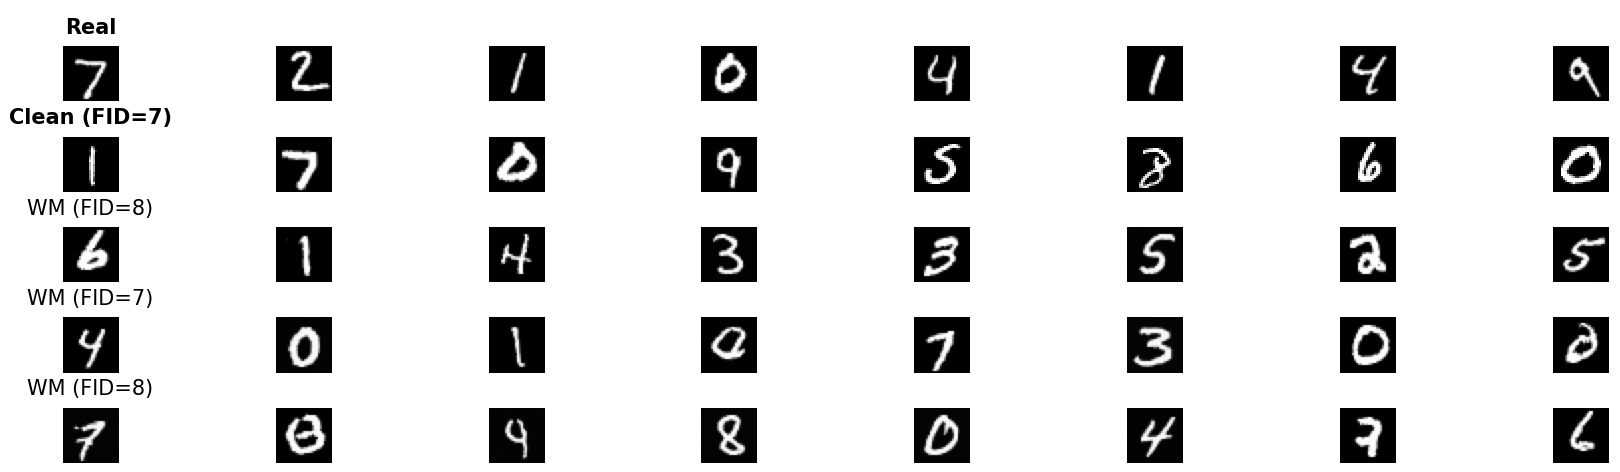
\includegraphics[width=\textwidth]{outputs/mnist_lora_results.png}
\caption{Generated MNIST samples from UNet + LoRA models.
Top row: real MNIST digits. Second row: clean UNet model.
Rows 3--5: watermarked LoRA models.}
\label{fig:samples_mnist_unet}
\end{figure}

\begin{figure}[h]
\centering
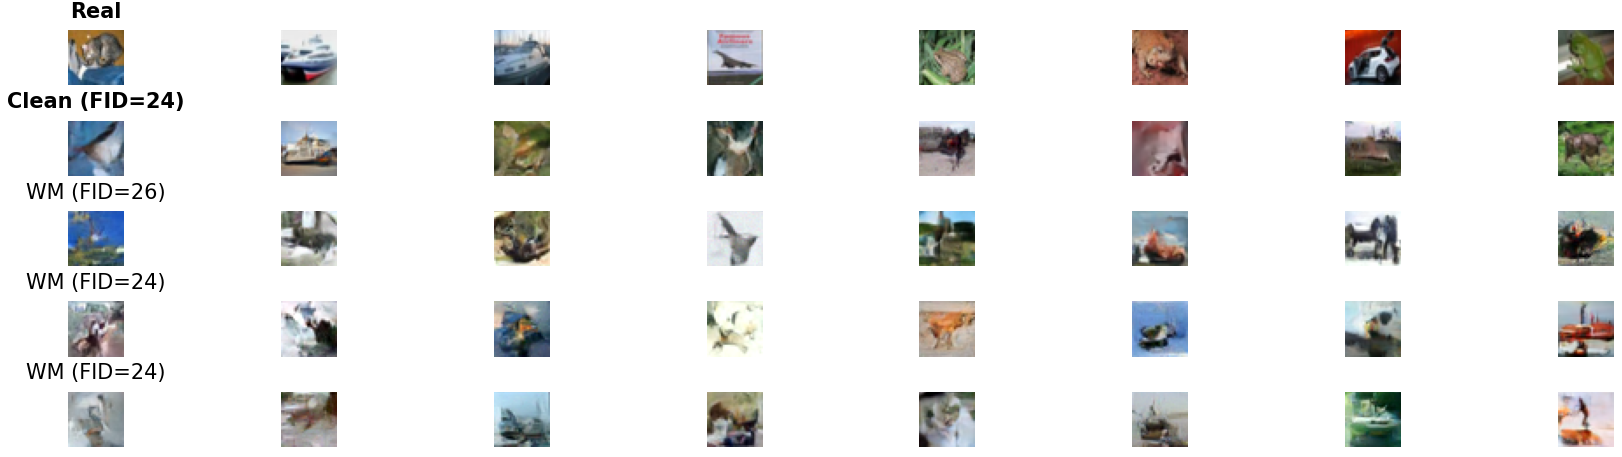
\includegraphics[width=\textwidth]{outputs/cifar10_lora_results.png}
\caption{Generated CIFAR-10 samples from UNet + LoRA models.
Top row: real CIFAR-10 images. Second row: clean UNet model.
Rows 3--5: watermarked LoRA models.}
\label{fig:samples_cifar10}
\end{figure}

\section{Hyperparameters}\label{app:hyperparams}

\begin{table}[h]
\centering
\caption{Complete hyperparameter configuration for all experiments.}
\label{tab:hyperparams}
\begin{tabular}{lcccc}
\toprule
Hyperparameter & MNIST (MLP) & MNIST (MLP 10K) & MNIST (UNet) & CIFAR-10 (UNet) \\
\midrule
\multicolumn{5}{c}{\textit{Data}} \\
\quad Image size & $28 \times 28$ (gray) & $28 \times 28$ (gray) & $28 \times 28$ (gray) & $32 \times 32$ (RGB) \\
\quad Training samples & $12{,}000$ & $12{,}000$ & $60{,}000$ & $50{,}000$ \\
\midrule
\multicolumn{5}{c}{\textit{Architecture}} \\
\quad Model & 4-layer MLP & 4-layer MLP & UNet & UNet \\
\quad Hidden size / ch. & $1{,}024$ & $1{,}024$ & 64--256 & 64--256 \\
\quad Activation & SiLU & SiLU & SiLU & SiLU \\
\quad LoRA rank & -- & -- & 4 & 4 \\
\quad LoRA $\alpha$ & -- & -- & 8 & 8 \\
\midrule
\multicolumn{5}{c}{\textit{Flow Matching}} \\
\quad Interpolation & Linear & Linear & Linear & Linear \\
\quad Training steps (base) & $5{,}000$ & $10{,}000$ & $5{,}000$ & $5{,}000$ \\
\quad Training steps (WM) & $5{,}000$ & $10{,}000$ & $500$ (LoRA) & $500$ (LoRA) \\
\quad Batch size & $512$ & $512$ & $512$ & $512$ \\
\quad Learning rate & $10^{-3}$ & $10^{-3}$ & $10^{-3}$ & $10^{-3}$ \\
\quad Optimizer & AdamW & AdamW & AdamW & AdamW \\
\midrule
\multicolumn{5}{c}{\textit{Watermark}} \\
\quad Projection dim.\ $k$ & 32 & 32 & 32 & 32 \\
\quad Message bits $L$ & 5 & 5 & 5 & 5 \\
\quad Strength $\epsilon_0$ & 0.3 & 0.2 & 0.2 & 0.2 \\
\quad Loss weight $\lambda$ & 0.02 & 0.018 & 0.01 & 0.01 \\
\midrule
\multicolumn{5}{c}{\textit{Detection}} \\
\quad Query budget $N$ & $4{,}096$ & $4{,}096$ & $4{,}096$ & $4{,}096$ \\
\quad Query distribution & $\mathcal{N}(0, 4I)$ & $\mathcal{N}(0, 4I)$ & $\mathcal{N}(0, 4I)$ & $\mathcal{N}(0, 4I)$ \\
\quad Time sampling & $\text{Uniform}(0,1)$ & $\text{Uniform}(0,1)$ & $\text{Uniform}(0,1)$ & $\text{Uniform}(0,1)$ \\
\midrule
\multicolumn{5}{c}{\textit{Evaluation}} \\
\quad Watermarked models & 6 & 6 & 3 & 3 \\
\quad Clean models & 2 & 2 & 1 & 1 \\
\quad Trials per model & 20 & 20 & 20 & 20 \\
\bottomrule
\end{tabular}
\end{table}

\end{document}

